% IEEE conference-style editable source. Build with IEEEtran.cls, pdflatex and BibTeX.
\documentclass[conference]{IEEEtran}
\usepackage{graphicx,booktabs,array,url}
\graphicspath{{figures/}}
\title{Design and Verification of an 8-Lane SIMD Vector Processing Unit Using Verilog HDL}
\author{\IEEEauthorblockN{Bulbul Agarwalla, Kanchan Rani, Kanishka Dubey, Shourya Pratap, and Udit Jain}
\IEEEauthorblockA{Department of Computer Science, Newton School of Technology, Rishihood University\\Subject: Modern Computer Architecture\\Faculty guide: [name/designation]\\Phase I report; deadline November 16, 2026, 11:59 PM IST (confirm actual submission date)}}
\begin{document}\maketitle
\begin{abstract}
Single instruction, multiple data (SIMD) processing applies one operation to several independent data elements, exposing data-level parallelism in a regular hardware structure. This project designs and verifies an eight-lane SIMD vector processing unit in Verilog HDL. The datapath accepts two 64-bit vectors, divides each into eight 8-bit lanes, and evaluates the same operation concurrently in eight combinational arithmetic logic units (ALUs). A pair of synchronous 64-bit operand registers, an opcode control unit, and an integrated processor top module provide registered input storage and coordinated execution. The ALUs implement 8-bit addition and subtraction, bitwise AND and OR, and unsigned less-than comparison; arithmetic results are retained at eight bits. Unsupported 3-bit opcodes are flagged invalid and the integrated result is masked to zero. Verification with Icarus Verilog 13.0 used module-level and integrated testbenches. Five counter-based benches reported 1,301 passing checks: 1,023 register, 184 SIMD datapath, 8 control, 6 scalar-comparison, and 80 integrated checks. The basic ALU and SIMD benches are display-oriented. Simulation establishes behavior for exercised cases; no FPGA synthesis, resource utilization, maximum-frequency, or physical speedup measurement is available. A scalar reference model takes eight modeled cycles to process eight elements, while the SIMD datapath evaluates all lanes combinationally; this comparison illustrates parallel organization rather than measured hardware performance.
\end{abstract}
\begin{IEEEkeywords}SIMD, vector processing, Verilog HDL, arithmetic logic unit, RTL verification, computer architecture.\end{IEEEkeywords}
\section{Introduction}
Computer systems exploit parallelism at multiple levels. SIMD is a data-parallel organization in which one operation or control decision applies to multiple data values. Flynn's taxonomy distinguishes SIMD from scalar and multiple-instruction organizations \cite{flynn1972}. Vector processors developed this principle for ordered elements and vector functional units \cite{russell1978}. This project implements the idea at modest scale: two 64-bit operands are treated as eight byte-wide elements, and eight 8-bit ALUs perform the selected operation concurrently.

The objectives are to implement an eight-lane datapath, two 64-bit operand registers, a 3-bit opcode decoder, an integrated top module, and functional tests. The scope is RTL and simulation; it excludes an FPGA build, physical implementation, pipeline, memory system, and measured hardware performance. Contributions are the parameter-free 8-by-8-bit datapath, separate storage and control, integrated wrapper, and testbenches from module smoke tests to integrated assertions. A scalar loop model compares result vectors with SIMD evaluation; no novelty in SIMD theory is claimed.
\section{Related Work}
Flynn's classification frames the shared-control, multiple-data organization used here \cite{flynn1972}. Russell describes the CRAY-1 vector system, a significant historical example of vector registers and functional units \cite{russell1978}. The present design is smaller and omits vector length, chaining, memory subsystems, and pipelining. Computer architecture texts analyze performance through execution time, throughput, and parallelism rather than replicated unit count alone \cite{hennessy2017}; Amdahl's law shows that speedup depends on the parallelizable fraction \cite{amdahl1967}. Therefore the scalar/SIMD comparison here is not interpreted as an achieved eightfold speedup.

Verilog is standardized as a hardware description language for modeling digital systems \cite{ieee1364}. RTL simulation can check behavior but does not establish physical timing or FPGA utilization. This project uses Icarus Verilog, an open-source simulator \cite{icarus}, for compile-and-run tests. Test strategies combine directed boundary cases, reset/write behavior, decoding, and result comparisons; failure policies differ among benches and are reported explicitly.
\section{Problem and Architecture}
Given 64-bit vectors $A$ and $B$, lane $i$ is $A[8i+7:8i]$ and $B[8i+7:8i]$, for $i\in\{0,\ldots,7\}$. The result byte occupies $R[8i+7:8i]$; lane 0 is least significant. Fig.~\ref{fig:integrated} shows register, control, and datapath paths.
\begin{figure}[t]\centering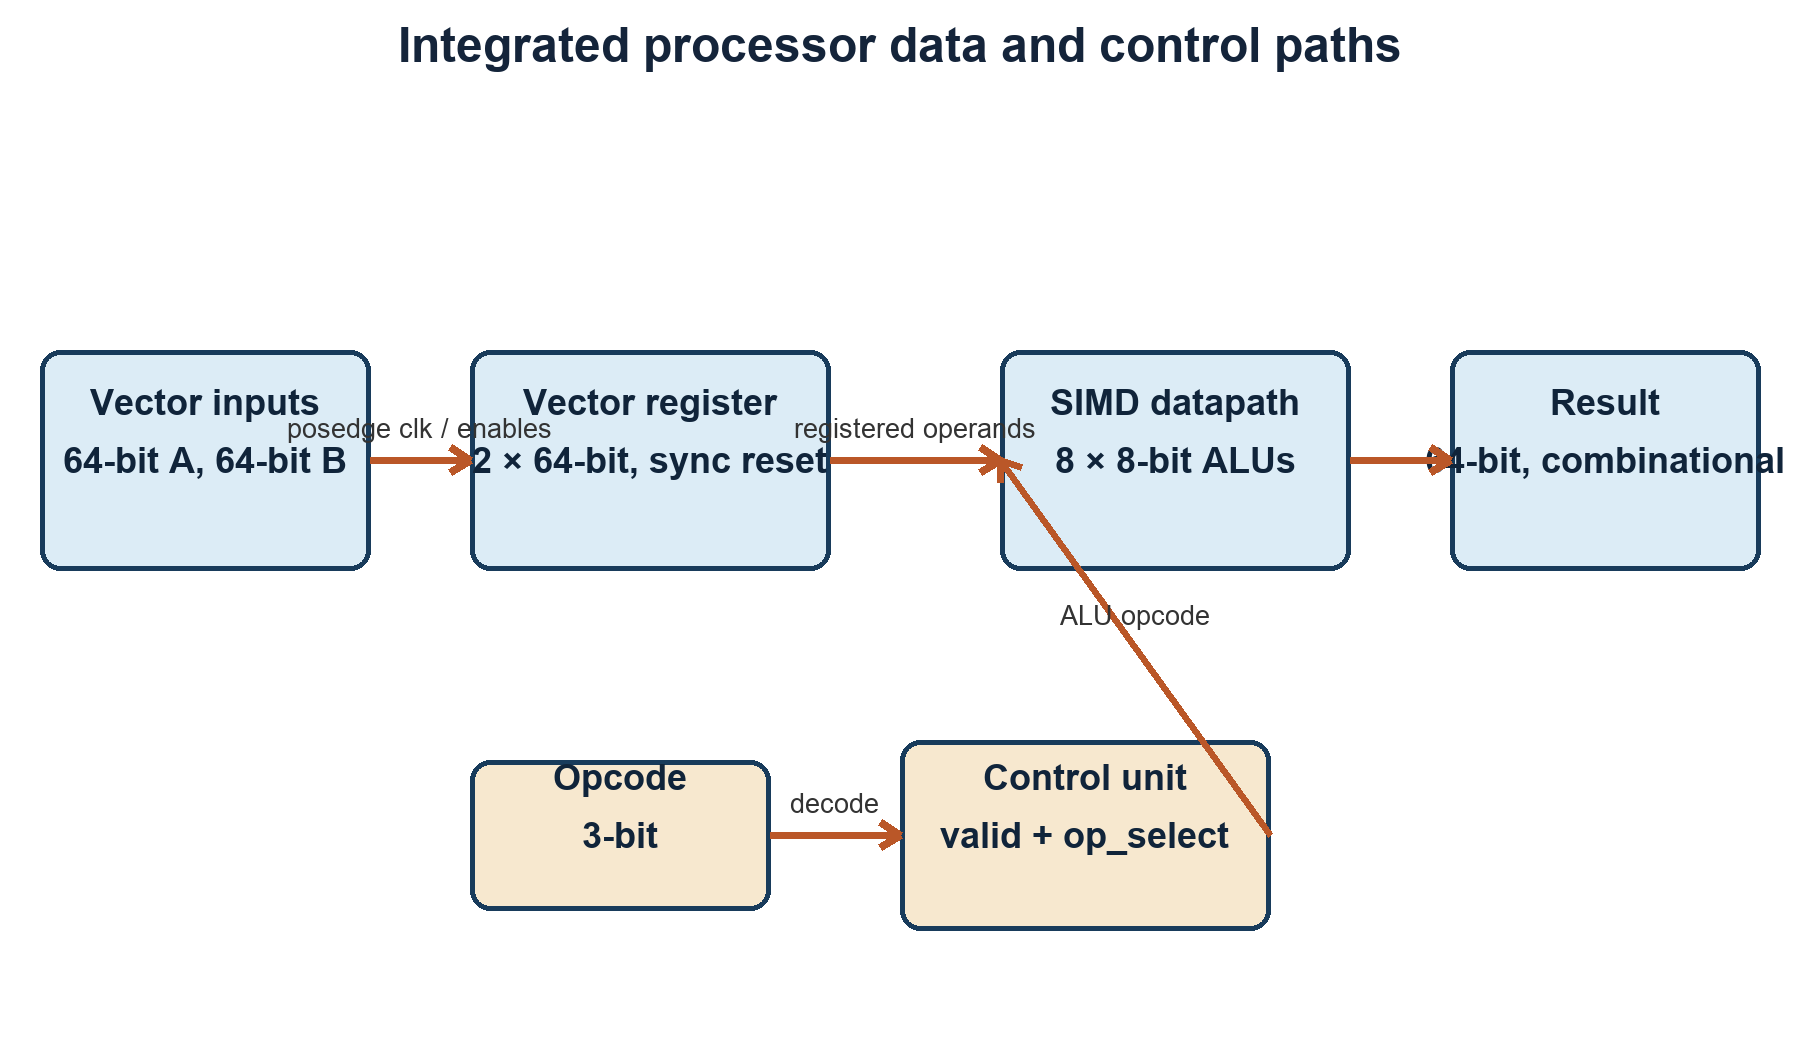
\includegraphics[width=\columnwidth]{integrated_architecture.png}\caption{Integrated register, control, and datapath connections. Result is combinational after operands and opcode settle.}\label{fig:integrated}\end{figure}
At a rising edge, vector\_register captures A and/or B using independent enables. The control unit decodes the external opcode combinationally. simd\_processor\_top connects registered operands and decoded ALU opcode to simd\_top. The result is combinational, not captured in an output register. When operation\_valid is low, the integrated top masks the result to zero. Fig.~\ref{fig:lanes} shows byte ordering.
\begin{figure}[t]\centering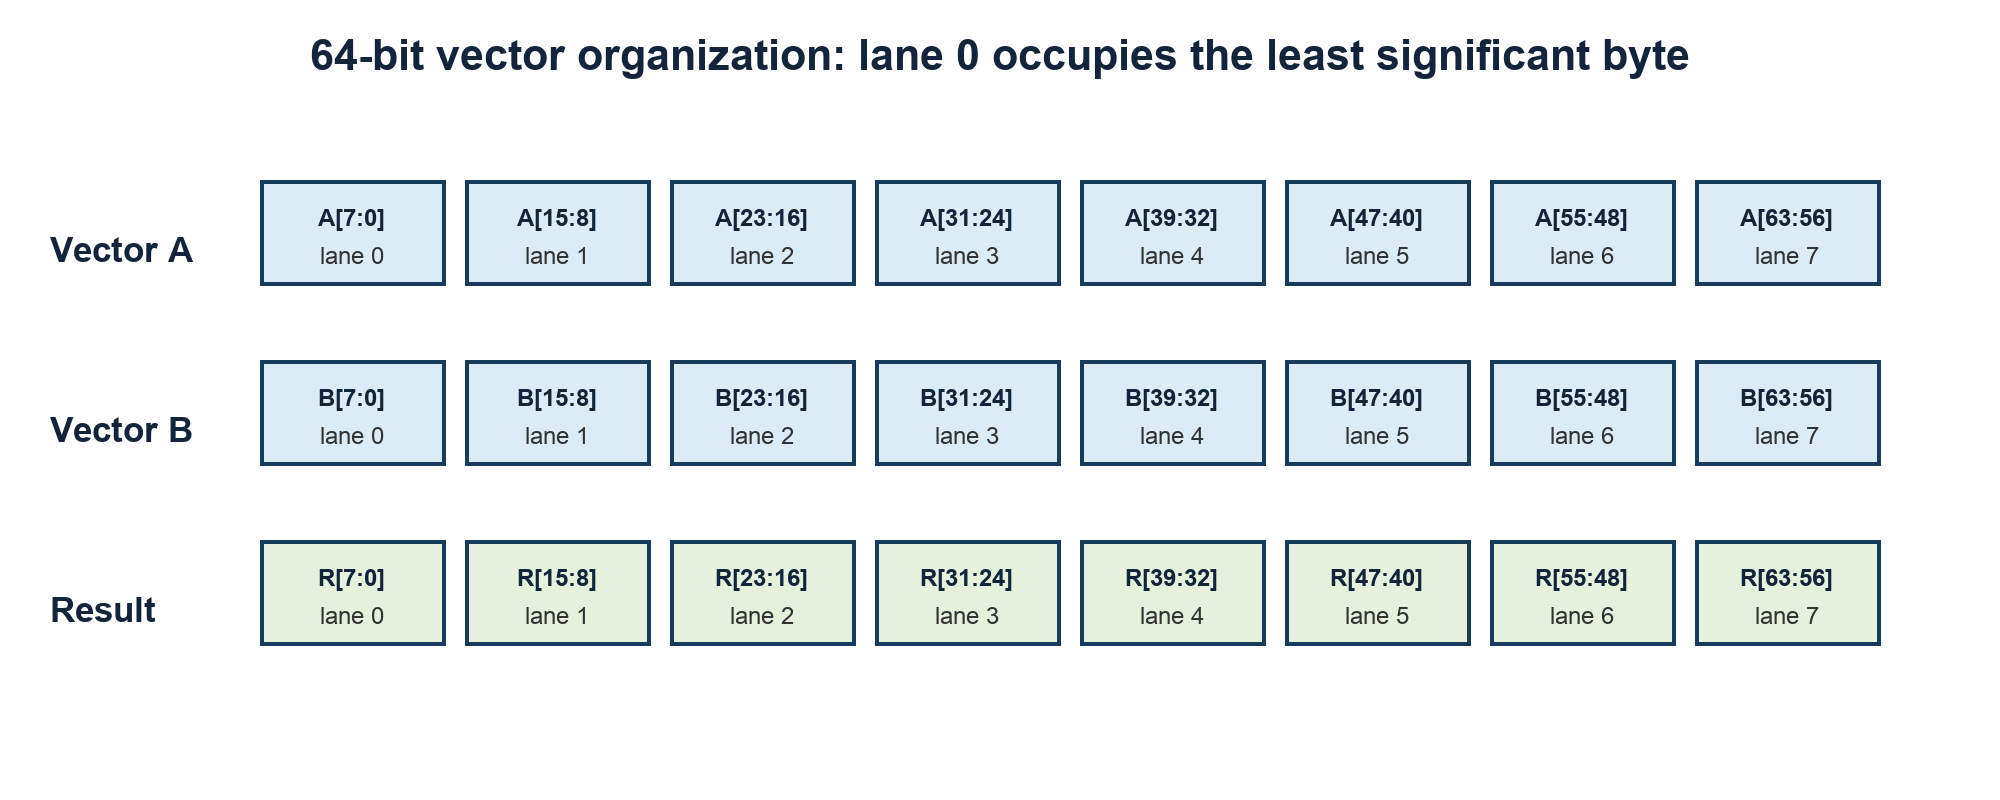
\includegraphics[width=\columnwidth]{lane_mapping.png}\caption{Byte lane mapping; lane 0 occupies bits [7:0].}\label{fig:lanes}\end{figure}
Each ALU has unsigned 8-bit inputs, 3-bit opcode and 8-bit result. ADD/SUB retain the least significant eight bits; carry/borrow is not exposed. LT is unsigned and returns 8'h01 if $A<B$, else 8'h00. The opcode table is in Table~\ref{tab:ops}.
\begin{table}[t]\caption{Supported operations}\label{tab:ops}\centering\begin{tabular}{lll}\toprule Operation&Opcode&Behavior\\\midrule ADD&000&$(A+B)\bmod 256$\\SUB&001&$(A-B)\bmod 256$\\AND&010&bitwise $A\ \&\ B$\\OR&011&bitwise $A\ |\ B$\\LT&100&unsigned $A<B?1:0$\\Reserved&101--111&invalid; masked result zero\\\bottomrule\end{tabular}\end{table}
The two 64-bit registers use active-high synchronous reset, which clears both at a rising edge and takes priority over writes. Otherwise the independent enables update each register; disabled registers retain state, and simultaneous updates are supported. The decoder emits a 5-bit one-hot op\_select (bits 0--4 map ADD, SUB, AND, OR, LT), valid, and safe ALU opcode. Encodings 101--111 clear valid and op\_select and select safe opcode 000.
\section{RTL Implementation}
The hierarchy is shown in Fig.~\ref{fig:hier}. simd\_top uses a generate loop for eight ALU instances and byte part-selects $[i*8 +: 8]$. The integrated top wires sequential storage, combinational decode, and combinational execution. opcode\_defs.vh contains guarded opcode constants.
\begin{figure}[t]\centering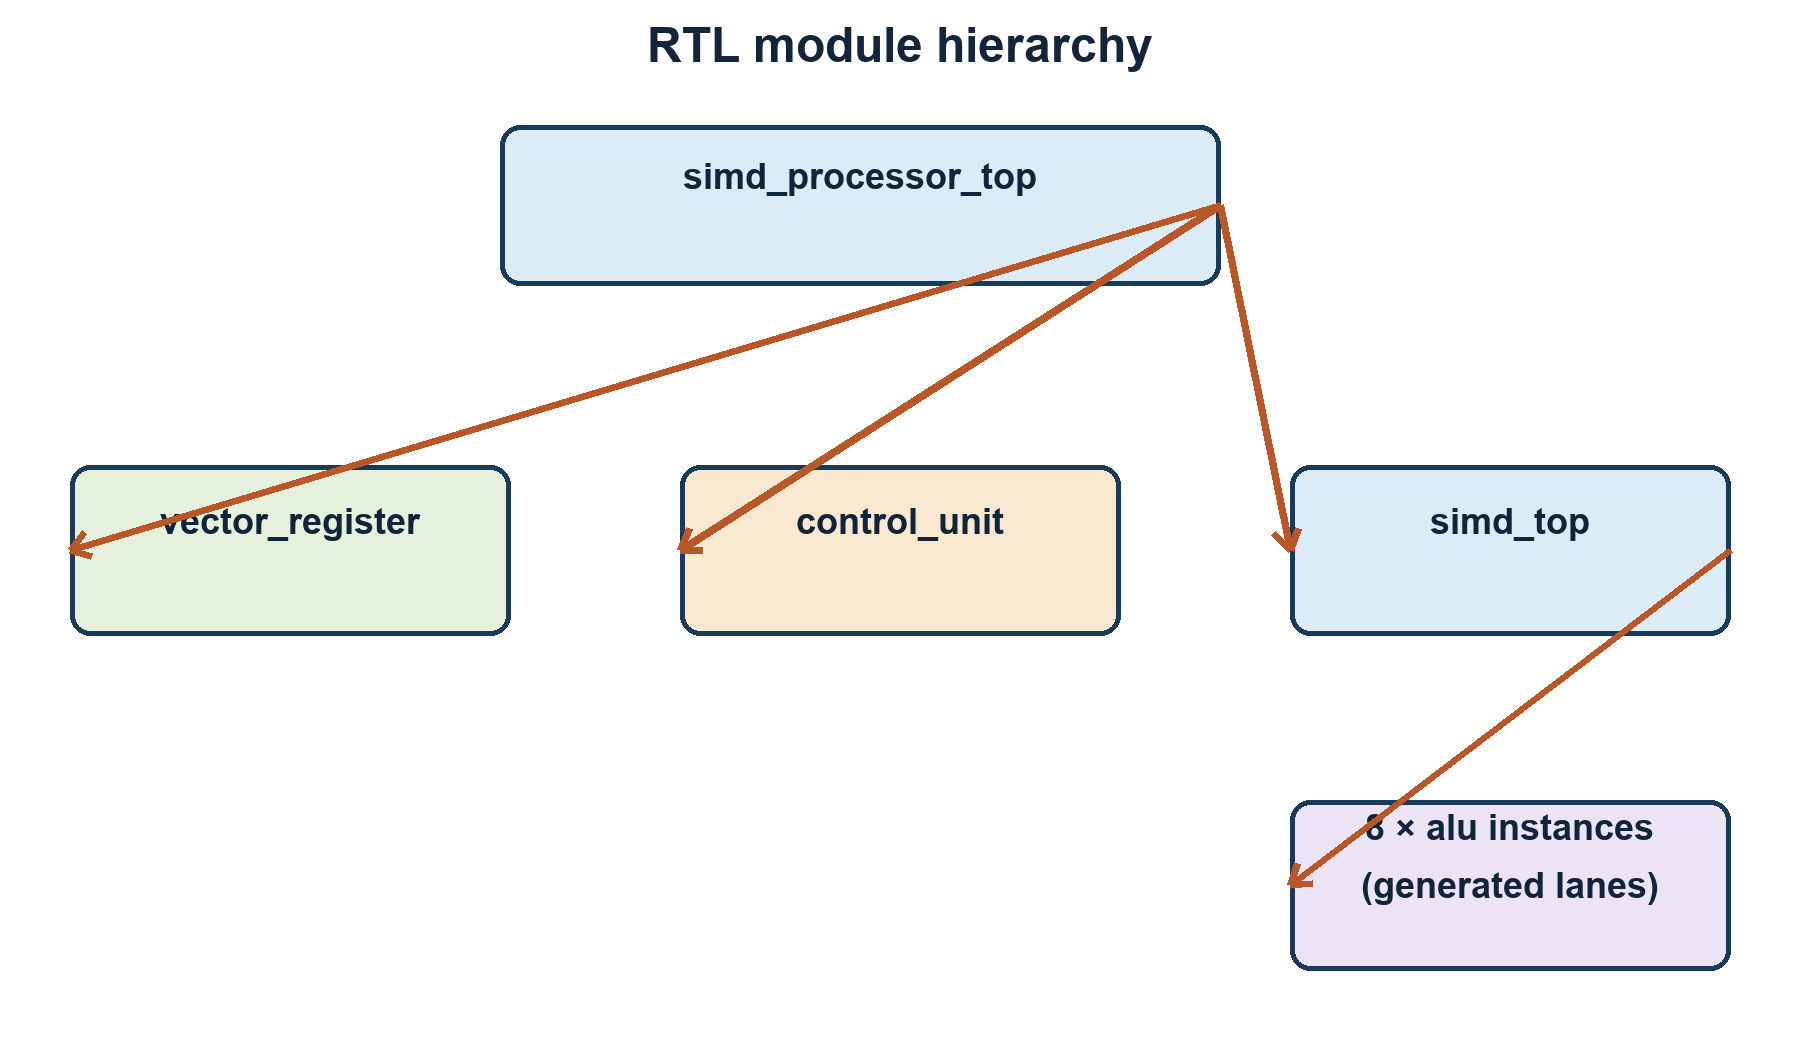
\includegraphics[width=\columnwidth]{module_hierarchy.png}\caption{RTL module hierarchy. Eight ALU instances are generated within simd\_top.}\label{fig:hier}\end{figure}
\begin{table}[t]\caption{Major RTL modules}\centering\begin{tabular}{@{}p{.34\columnwidth}p{.53\columnwidth}@{}}\toprule Module&Responsibility\\\midrule alu&8-bit combinational ALU with five operations\\vector\_register&Two 64-bit operands, synchronous reset, independent enables\\simd\_top&Eight parallel byte ALUs and packed 64-bit result\\control\_unit&Opcode decode, valid, one-hot operation selection\\simd\_processor\_top&Integration and invalid-result mask\\opcode\_defs.vh&Guarded operation constants\\\bottomrule\end{tabular}\end{table}
Simulation used Icarus Verilog 13.0 with \texttt{iverilog -g2012 -Wall} and \texttt{vvp}; the rerun produced no compiler warnings. A stored operand becomes visible after the active edge; its result then settles through combinational decode and lane logic without a result-register edge.
\section{Verification Methodology}
Directed tests exercise operations, invalid opcodes, register writes and holds, synchronous reset, lane order, arithmetic wraparound, comparison boundaries, and integrated opcode changes. Fig.~\ref{fig:verify} summarizes the workflow.
\begin{figure}[t]\centering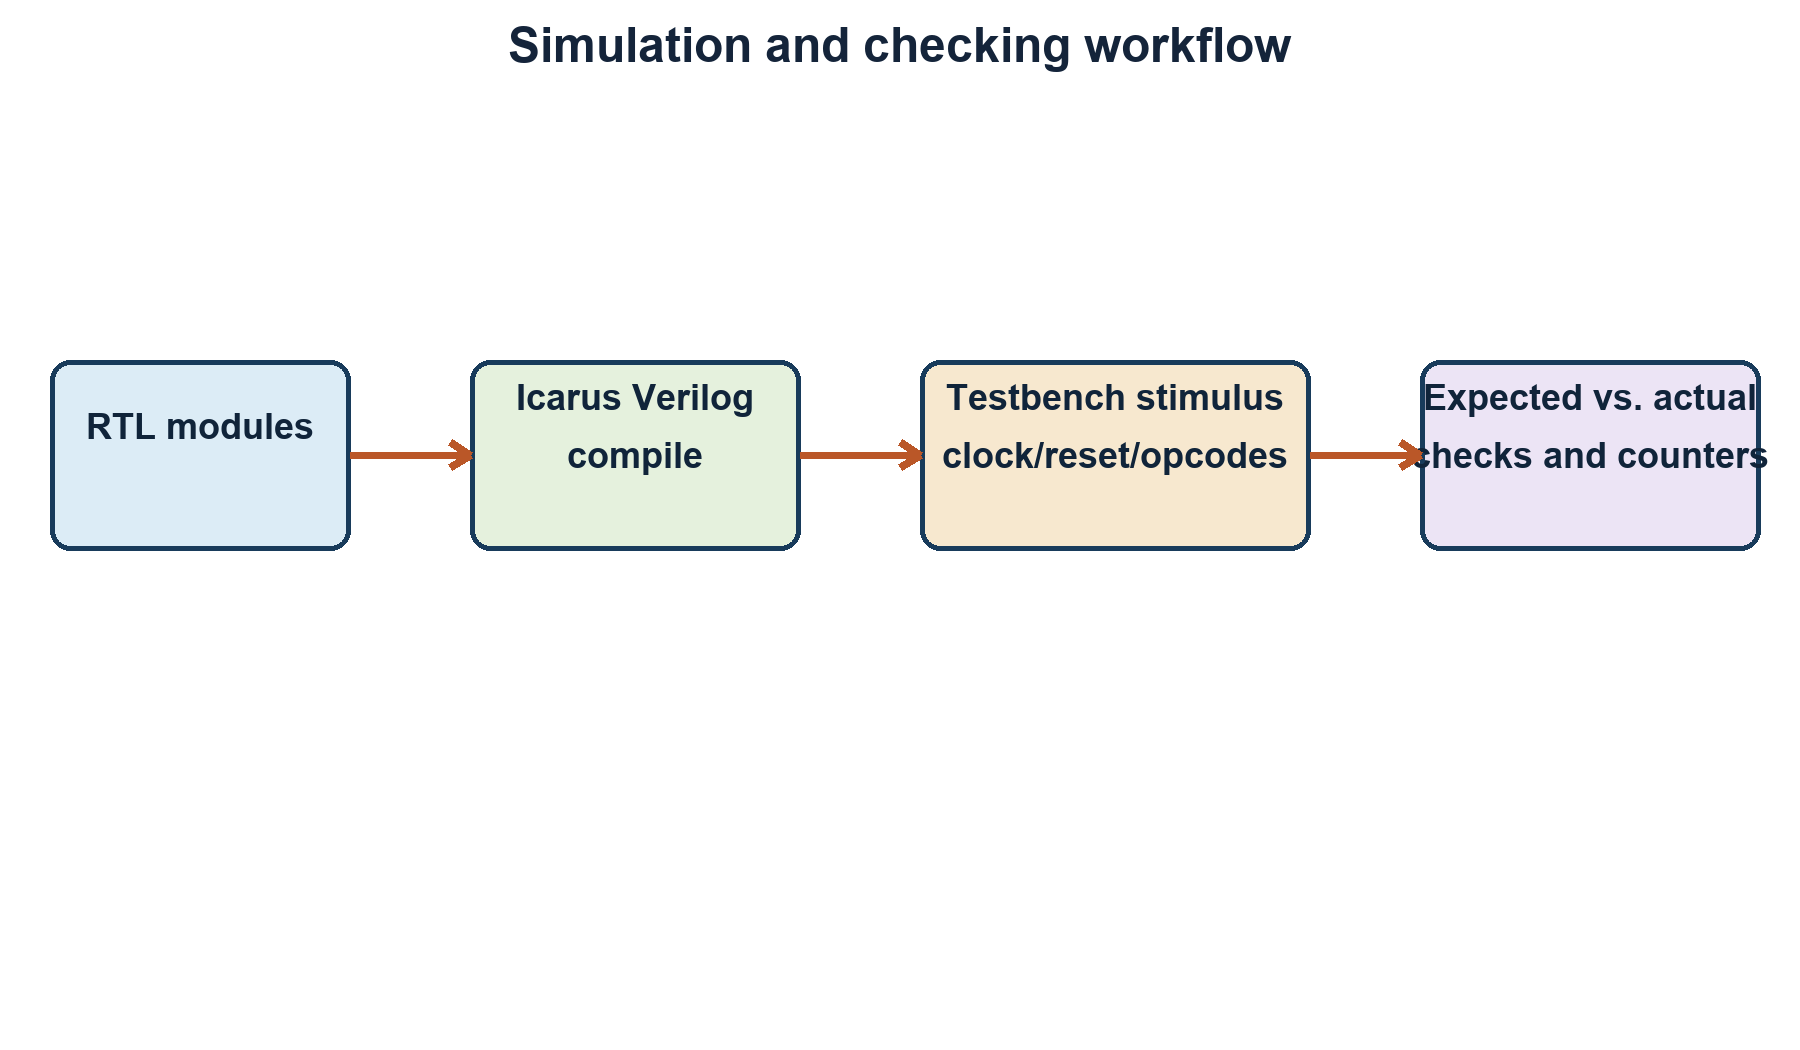
\includegraphics[width=\columnwidth]{verification_flow.png}\caption{Compile, stimulus, and checking workflow.}\label{fig:verify}\end{figure}
\begin{table}[t]\caption{Verification outcomes observed in the rerun}\centering\footnotesize\begin{tabular}{@{}p{.30\columnwidth}p{.18\columnwidth}p{.40\columnwidth}@{}}\toprule Bench&Pass / fail&\shortstack{Coverage /\\failure handling}\\\midrule Register&1,023 / 0&Reset, enables, hold, lanes, boundaries, randomized model; fatal mismatch\\SIMD verification&184 / 0&SIMD operations and lane cases; fatal mismatch\\Control unit&8 / 0&Five legal and three invalid decodes; counters then finish\\Scalar comparison&6 / 0&Five operations and invalid equivalence; counters then finish\\Integrated processor&80 / 0&Reset, writes, opcodes, results; fatal mismatch\\ALU; SIMD smoke&Display&Smoke demonstrations; not assertion checks\\Scalar performance&1 comparison&Eight modeled cycles; prints status, no fatal mismatch\\\bottomrule\end{tabular}\end{table}
The five counter-based suites sum to 1,301 reported passing checks, not exhaustive coverage or formal verification. control\_tb and scalar\_tb print failures but call \$finish regardless; scalar\_performance\_tb also prints status without a fatal mismatch path. register\_tb, simd\_verification\_tb, and integrated top tests use \$fatal on mismatches.
\section{Results and Discussion}
The rerun compiled and executed the benches with zero return codes. Results demonstrate byte-wise ADD, SUB, AND, OR and unsigned LT, register reset/write/hold behavior, invalid opcode flagging and output masking, and integrated operation. The testbenches combine directed and randomized cases but do not test every possible combination. Fig.~\ref{fig:wave} reproduces the existing register waveform evidence.
\begin{figure}[t]\centering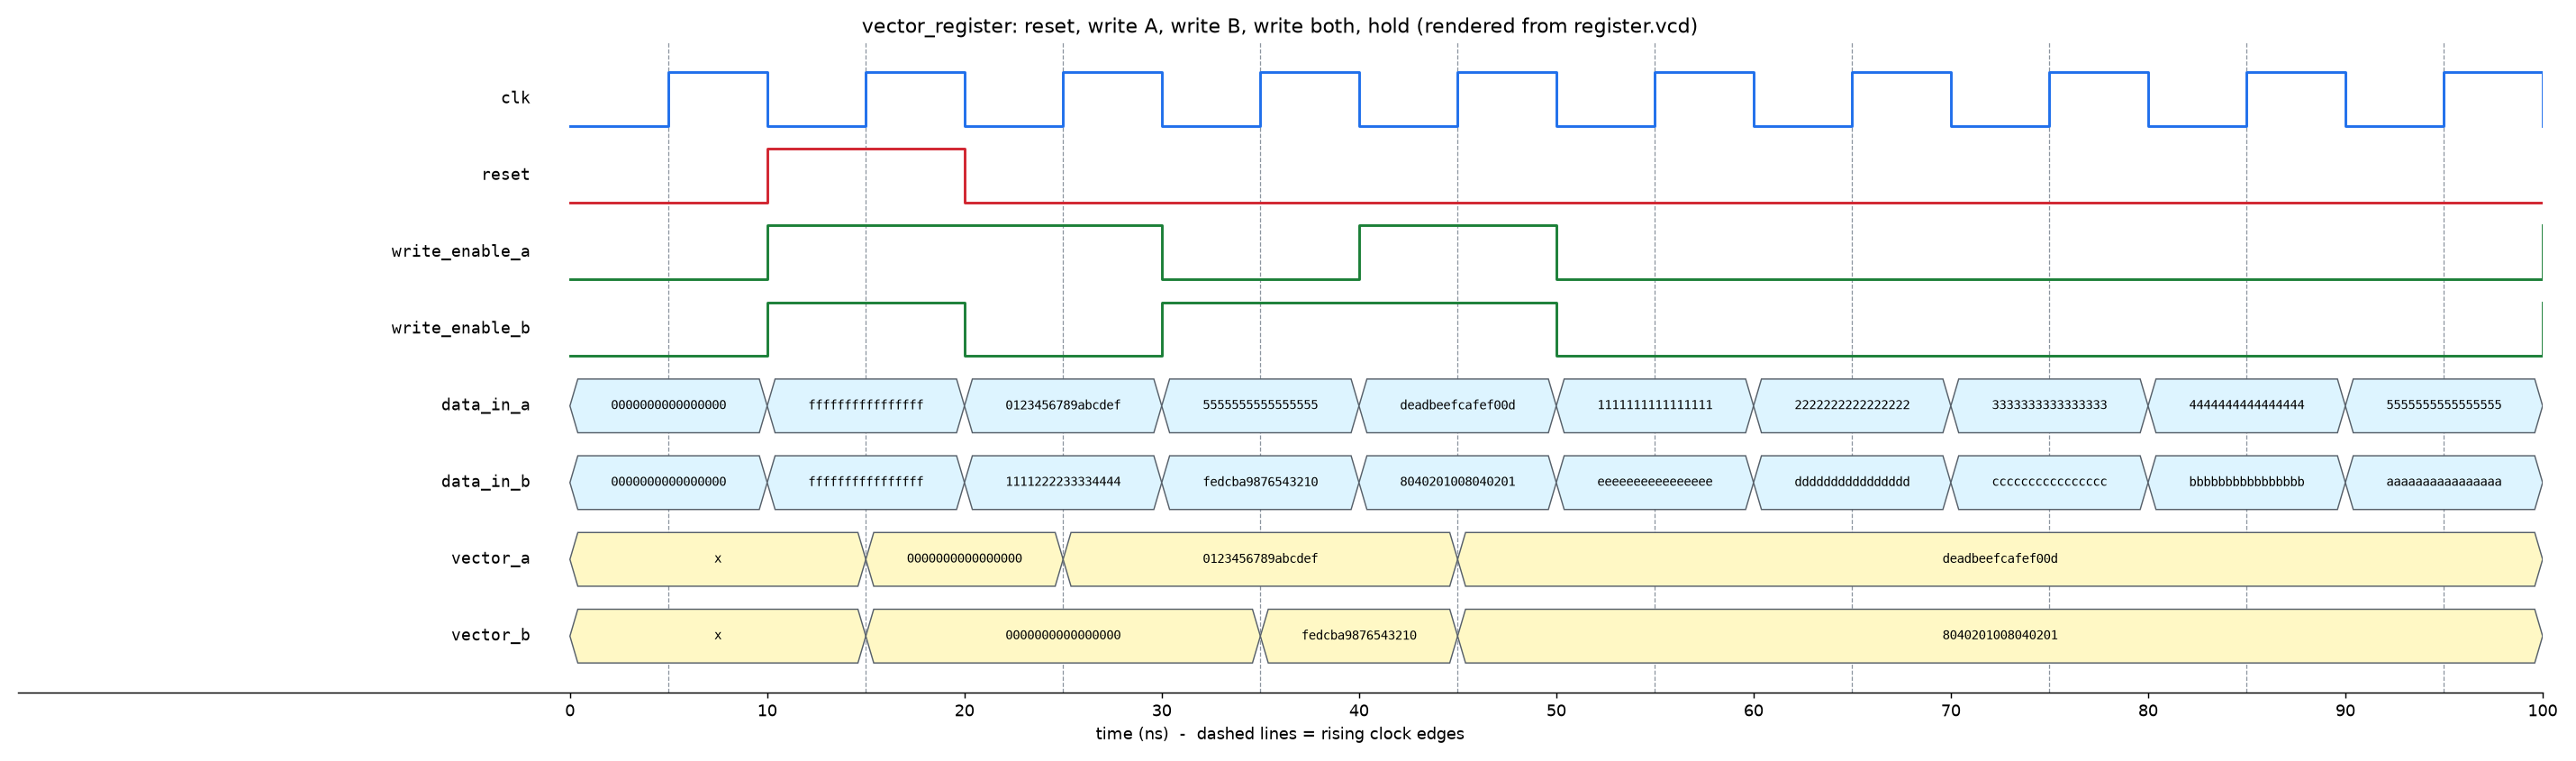
\includegraphics[width=\columnwidth]{register_waveform.png}\caption{Existing project waveform capture showing clock, synchronous reset, write enables, inputs, and registered outputs.}\label{fig:wave}\end{figure}
The scalar comparison loops over the eight bytes and compares its packed result with simd\_top for five supported operations and invalid opcode 101. scalar\_performance\_tb models one scalar ALU over eight clocked iterations, while SIMD evaluates all eight lanes combinationally. Eight model cycles versus one combinational evaluation is an abstract comparison; it does not establish equivalent clock periods, critical paths, throughput, or physical 8-times speedup.
No FPGA synthesis/implementation reports, resource utilization, maximum frequency, timing slack, power, or physical performance measurements are available. Actual timing depends on synthesis, target, constraints, and implementation.
\section{Team Contributions}
Git history contains five repository identities. Authorship supports evidence of recorded commits, not full allocation. Confirm all scopes and official names before submission.
\par\medskip\noindent\refstepcounter{table}\begin{minipage}{\columnwidth}\centering{\footnotesize\textbf{TABLE \thetable}\\Contributions based on repository evidence\par}\smallskip\footnotesize\begin{tabular}{@{}p{.35\columnwidth}p{.51\columnwidth}@{}}\toprule \shortstack{Team member /\\enrollment no.}&Evidence and confirmation\\\midrule \shortstack{Bulbul Agarwalla\\2401010131}&Author of initial SIMD core and integrated processor work; confirm scope.\\\shortstack{Kanchan Rani\\2401010206}&Git identity kanchan97-cp; authored performance-analysis commit; confirm scope.\\\shortstack{Kanishka Dubey\\2401010208}&Author of SIMD testbench/results work; confirm scope.\\\shortstack{Shourya Pratap\\2401010445}&Author of control/opcode/control-test work; confirm scope.\\\shortstack{Udit Jain\\2401010482}&Author of register/register-test/evidence work; confirm scope.\\\bottomrule\end{tabular}\end{minipage}\par\medskip
\section{Conclusion and Future Work}
The integrated unit joins two synchronous 64-bit operand registers, an opcode decoder, and eight parallel byte ALUs. It supports ADD, SUB, AND, OR, and unsigned LT; invalid opcodes are flagged and masked. Five counter-based suites reported 1,301 passing checks, including 80 integrated checks. This establishes tested RTL behavior, not FPGA implementation, resource use, timing, or hardware speedup.
Future work includes FPGA synthesis and timing/resource analysis, hardware validation, wider vectors, more operations, pipelining, stronger mismatch handling, and benchmarks under equivalent clock and workload assumptions.
\section*{Submission Notes}
Snapshot: main@94e7303 (Nov. 15, 2026). Add the faculty guide and actual submission date before submission.
\bibliographystyle{IEEEtran}\bibliography{references}
\end{document}
